\label{research}
So far, we discussed an extension of the pilot abstraction to support data analytics and task based data intensive applications on HPC resources, a comparison between different task-based data oriented frameworks, and a design comparison for scientific workflows.
In addition, we identified a need for the execution of scientific computational campaigns with minimum user intervention, independent from users' scientific domain.
In this section, we motivate and propose a Campaign Manager (CM) for creating and enacting a campaign execution plan.

\subsection{Motivation}
\label{subsec:motivation}
Campaigns from the biomolecular and earth sciences are diverse in terms of composition, number and size of workflow members, and dynamicity.
Biomolecular science campaigns may be comprised from a small number of workflows with millions of tasks, or thousands of workflows with tens to hundreds tasks~\cite{dakka2018high}. 
Earth sciences campaigns, especially those which use VHR satellite imagery, comprise of workflows with thousands of tasks.
The number of workflows depends on the number of images the user has access to as well as the time they are able to obtain imagery.
These workflows can be static~\cite{paraskevakos2019workflow} or dynamic~\cite{dakka2018high}.

Resource requirements of these campaigns are heterogeneous, in terms of number of resources required and type. 
Biomolecular science software tools support MPI/OpenMP, GPUs, and other accelerators, such as Intel Phi processors~\cite{cheatham2015impact} for executing either simulations or analysis.
In addition, some biomolecular analysis tool require data oriented frameworks, such as PMDA~\cite{fan2019pmda}.
Earth sciences applications, based on imagery, are creating workflows that are executing a series of CPU based preprocessing, and eventually execute a computer vision algorithm on GPUs~\cite{paraskevakos2019workflow}.
As a result, the user needs to manage different types of resources as well as resource requirements for each workflow.

Scientific computational campaign workflows can be executed on a number of HPC resources as long as they meet the workflows' computational requirements.
Despite the fact, users tend to execute all their workflows on one or two systems, under-utilizing their allocations and increasing the makespan of the campaign.
Being able to distribute workflows on different resources will increase the resource utilization of the campaign, but also provide opportunity for optimizing the execution time of the campaign.

Based on the above, there is a need for a system that supports the execution of campaign with heterogeneous resource requirements.
This system should allow users to describe a set of workflows with their computing requirements, the campaign's objective, a set of resources along with the allocations on those resources, and any other information the user deems important, for example workflow importance.
Based on this information, the system should be able to derive and enact an execution plan without any further user intervention.
As a result, users will be able to compile computational campaigns that allow them to execute scientific experiments to sizes prior unfeasible, at least in terms of number of workflows.


\subsection{Proposed Topic}

% ------------------------------------------------------------------------------
% Scientific campaings
Scientific workflows are generally described by a direct acyclic graph, where the nodes are tasks and the edges dependencies.
A subset of this general description of workflows are those which can be represented via the Pipeline, Stage, Task (PST) model~\cite{balasubramanian2018harnessing}.
The PST model describes workflows as a set of pipelines, where each pipeline is a sequence of stages.
Each stage then is a set of tasks that need to be executed.
Concurrency is achieved in the level of pipelines and the level of tasks. 
Based on our use cases, we particularly interested in scientific campaigns comprised by workflows that can be described via the PST model.
Figure~\ref{fig:bio_earth_workflows} shows two example workflows from the biomolecular sciences (Fig.~\ref{fig:bio_workflow}) and the earth sciences (Fig.~\ref{fig:earth_workflow}). 

\begin{figure*}[ht!]
    \centering
    \begin{subfigure}[b]{0.45\textwidth}
        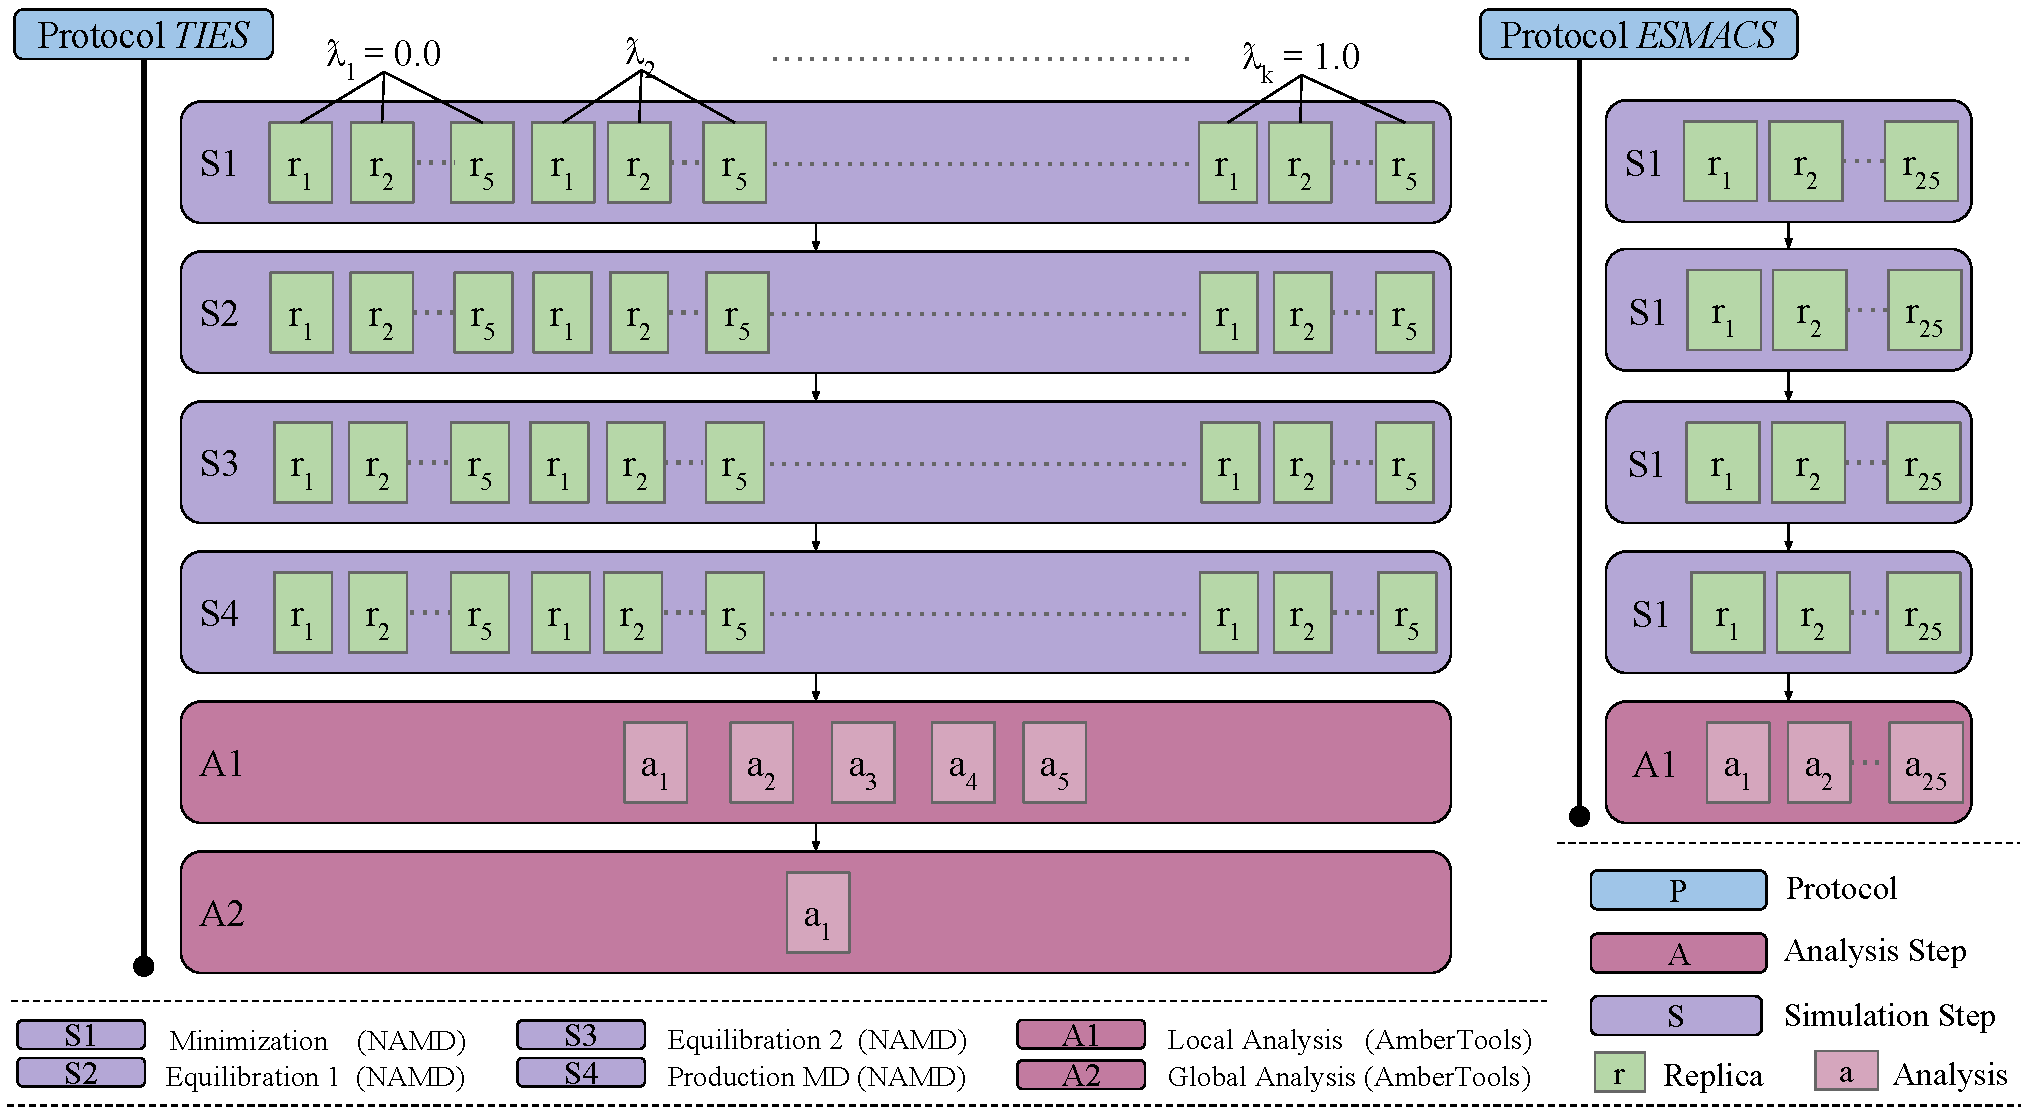
\includegraphics[width=\linewidth]{figures/bio_workflow.pdf}
        \caption{}
        \label{fig:bio_workflow}
    \end{subfigure}%
    ~ 
    \begin{subfigure}[b]{0.45\textwidth}
        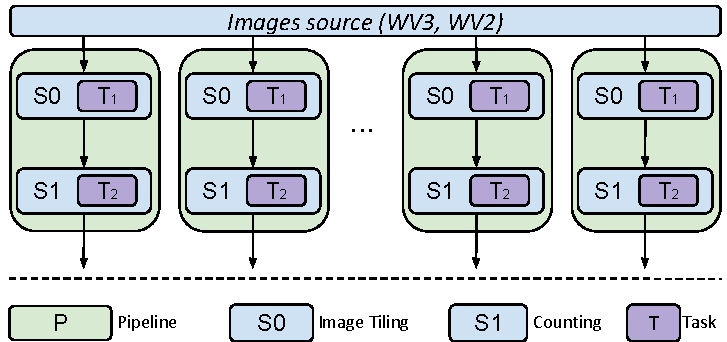
\includegraphics[width=\linewidth]{figures/earth_workflow.pdf}
        \caption{}
        \label{fig:earth_workflow}
    \end{subfigure}
    \caption{Biomolecular and Earth Science example workflows. \ref{fig:bio_workflow} Biomolecular workflow based on PST model example~\cite{dakka2018concurrent}; \ref{fig:earth_workflow} Earth science workflow based on PST model example~\cite{paraskevakos2019workflow}}\label{fig:bio_earth_workflows}
\end{figure*}


% ----------------------------------------------------------------------------
% campaign makespan modeling
Achieving a campaign computational objective, such as time to completion or throughput, would require calculating and optimizing the makespan of the campaign.
The makespan of a campaign is the time needed to execute all the workflows of the campaign, or alternatively, the maximum execution time among all paths throughout the campaign~\cite{chirkin2017execution}.
We propose to utilize and extend the Heterogeneous Earliest Finish Time (HEFT) algorithm~\cite{topcuoglu2002performance} algorithm.
HEFT is an offline scheduling algorithm which calculates the makespan of a workflow on heterogeneous resources.
HEFT uses a matrix to represent execution time of tasks on resources, assigning tasks to the resource that minimizes the finish time of the task, and has complexity proportional to the number of dependencies between tasks and the number of resources offered.
Furthermore, there has been some initial research to extend HEFT to resources that provide CPU and GPUs~\cite{shetti2013optimization}, as well as a method to extended HEFT on dynamic resources~\cite{dong2007pfas}.

There are several alternative methods and algorithms to calculate and optimize the makespan of a workflow~\cite{lu2019review}, including queuing networks~\cite{yao2019throughput,bao2019performance}, domain specific languages~\cite{carothers2017durango,maheshwari2016workflow}, and machine learning~\cite{witt2019predictive,pumma2017runtime}.
Queuing networks will be of limited use because they require from the user to provide a queuing network equivalent of the campaign.
A campaign is a set of workflows, and as a result having the user provide a queuing network representation of the campaign adds an additional layer of complexity.
Domain specific languages would require too much engineering effort to convert a workflow representation based on domain specific assumptions, e.g. MPI style workflow, or specific languages representation, e.g Swift, to a PST model representation.
Machine Learning approaches would require model training, validation and testing to produce a model.
In addition, since the execution is done on dynamic resources, the model should be retrained after every workflow execution.

% ----------------------------------------------------------------------------
% Initial Assumptions
Initially, we will assume a static campaign with static workflows, executing on static resources. 
This will allow us to understand the selected algorithm, and find its performance compared to a random plan.
Next, we will relax the assumption of static resources and work with dynamic resources.
We will introduce resource dynamicity as the availability of resources will be drawn from a binomial distribution.\gpnote{Binomial distribution is provides a yes or no outcome with p and q probabilities respectively. We need to find out how to select p and q, i.e. how often a resource is available compared to not.}
HEFT assumes static resources.
Introducing resource dynamicity requires to further extend HEFT to take into account resource availability to decide on which resources it will schedule workflows, as well as update the schedule as resource become unavailable.
In addition, we will try to further relax our assumptions and introduce dynamic campaigns, and dynamic workflows.
% ----------------------------------------------------------------------------
% Campaign Manager definition, requirements, features and capabilities
We propose to design a campaign manager (CM) which, given a campaign, an objective, and a set of constraints, can derive an execution plan by utilizing the proposed makespan HEFT method.
Execution planning for workflows are provided by Pegasus~\cite{deelman2015pegasus}, and ASKALON~\cite{fahringer2005askalon}.
We plan to extend these capability to campaigns.
Figure~\ref{fig:refarch} shows a reference architecture where the CM has two sub-components:
\begin{inparaenum}[(1)]
\item Makespan Calculator which implements HEFT, and
\item an Executor which executes the plan. 
\end{inparaenum}
Workflow execution will be done through an existing workflow management framework (WMF) on HPC resources.
If necessary, CM will adapt the execution plan by updating the workflows to resource mapping decisions. 
These updates will be based on workflows execution metrics provided by the selected WMF such as tasks execution time, overheads calculation and time to completion.
These metrics will be aggregated across workflows resulting in campaign-wide execution metrics.

\begin{figure*}[t]
    \centering
    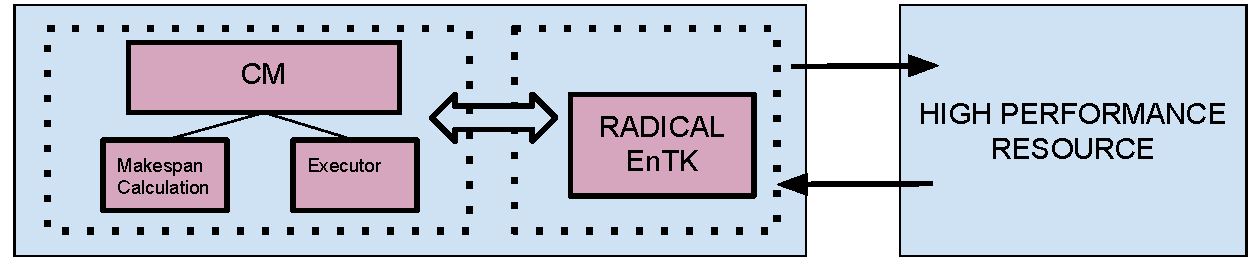
\includegraphics[width=.95\textwidth]{figures/CEM_RefArch.pdf}
    \caption{Reference Architecture of a Campaign Manager. Basic 
    subcomponents of Campaign Manager (CM): 1) Makespan Calculation, and 2) Executor. 
    CM communicates decisions to RADICAL-EnTK. CM communicates with HPCs to 
    execute parts of the campaign.}\label{fig:refarch}
\end{figure*}

The Makespan Calculator will be responsible for calculating and optimizing the makespan of a campaign based on a set of workflows, a set of resources, and the objective.
Calculating the makespan requires the calculator to have knowledge or derive of the execution time of the workflows that comprise the campaign on the available resources, as well as their availability.
HPC resources are dynamic, in the sense that their performance~\cite{pouchard2019computational} and availability fluctuates.
As a result, the Makespan Calculator requires to take into account performance fluctuations as workflows are being executed.
In addition, the Campaign Manager should be able to verify whether a resource is available and update the plan accordingly.

The Executor sub-component is responsible to execute, and monitor the plan by interfacing with a WMF.
Based on the plan the Makespan calculator decided, the Executor submits workflows to a WMF to execute on the selected resource.
This requires the Executor to work upon multiple workflows concurrently.
In addition, it should monitor workflow execution and resource availability.
An important requirement for the executor is to identify the reason of a failing workflow.
When the failure is because the resource is not available the specific workflow may need to be rescheduled and the plan to be updated.

RADICAL-Ensemble Toolkit~\cite{balasubramanian2018harnessing} (EnTK) is a workflow management framework.
We selected to utilize EnTK because it fits the requirements of the target use case as they are described in \S~\ref{subsec:motivation}
EnTK defines workflows as a set of pipelines, each pipeline is a sequence of stages, and in turn each stage a set of tasks.
EnTK support the execution of a sequence of workflows may either reuse resources or request new ones, based on how the user has programmed the application.
EnTK workflow execution is stateful, provides execution metrics, such as task execution time, and supports workflow execution on multiple HPC resources.
Furthermore, it support a pilot runtime system, RADICAL-Piliot~\cite{merzky2019using}, to execute workflows on HPC resources.
Pilot systems submit job placeholders on resources, and are able to execute tasks on the acquired resources.
The proposed campaign will interface with EnTK to execute workflows based on derived execution plan.
